\chapter{Setup Beaglebone Black mit CAN Cape}
\label{chap:setupbeaglebone}

\begin{figure}[hbtp]
    \center
    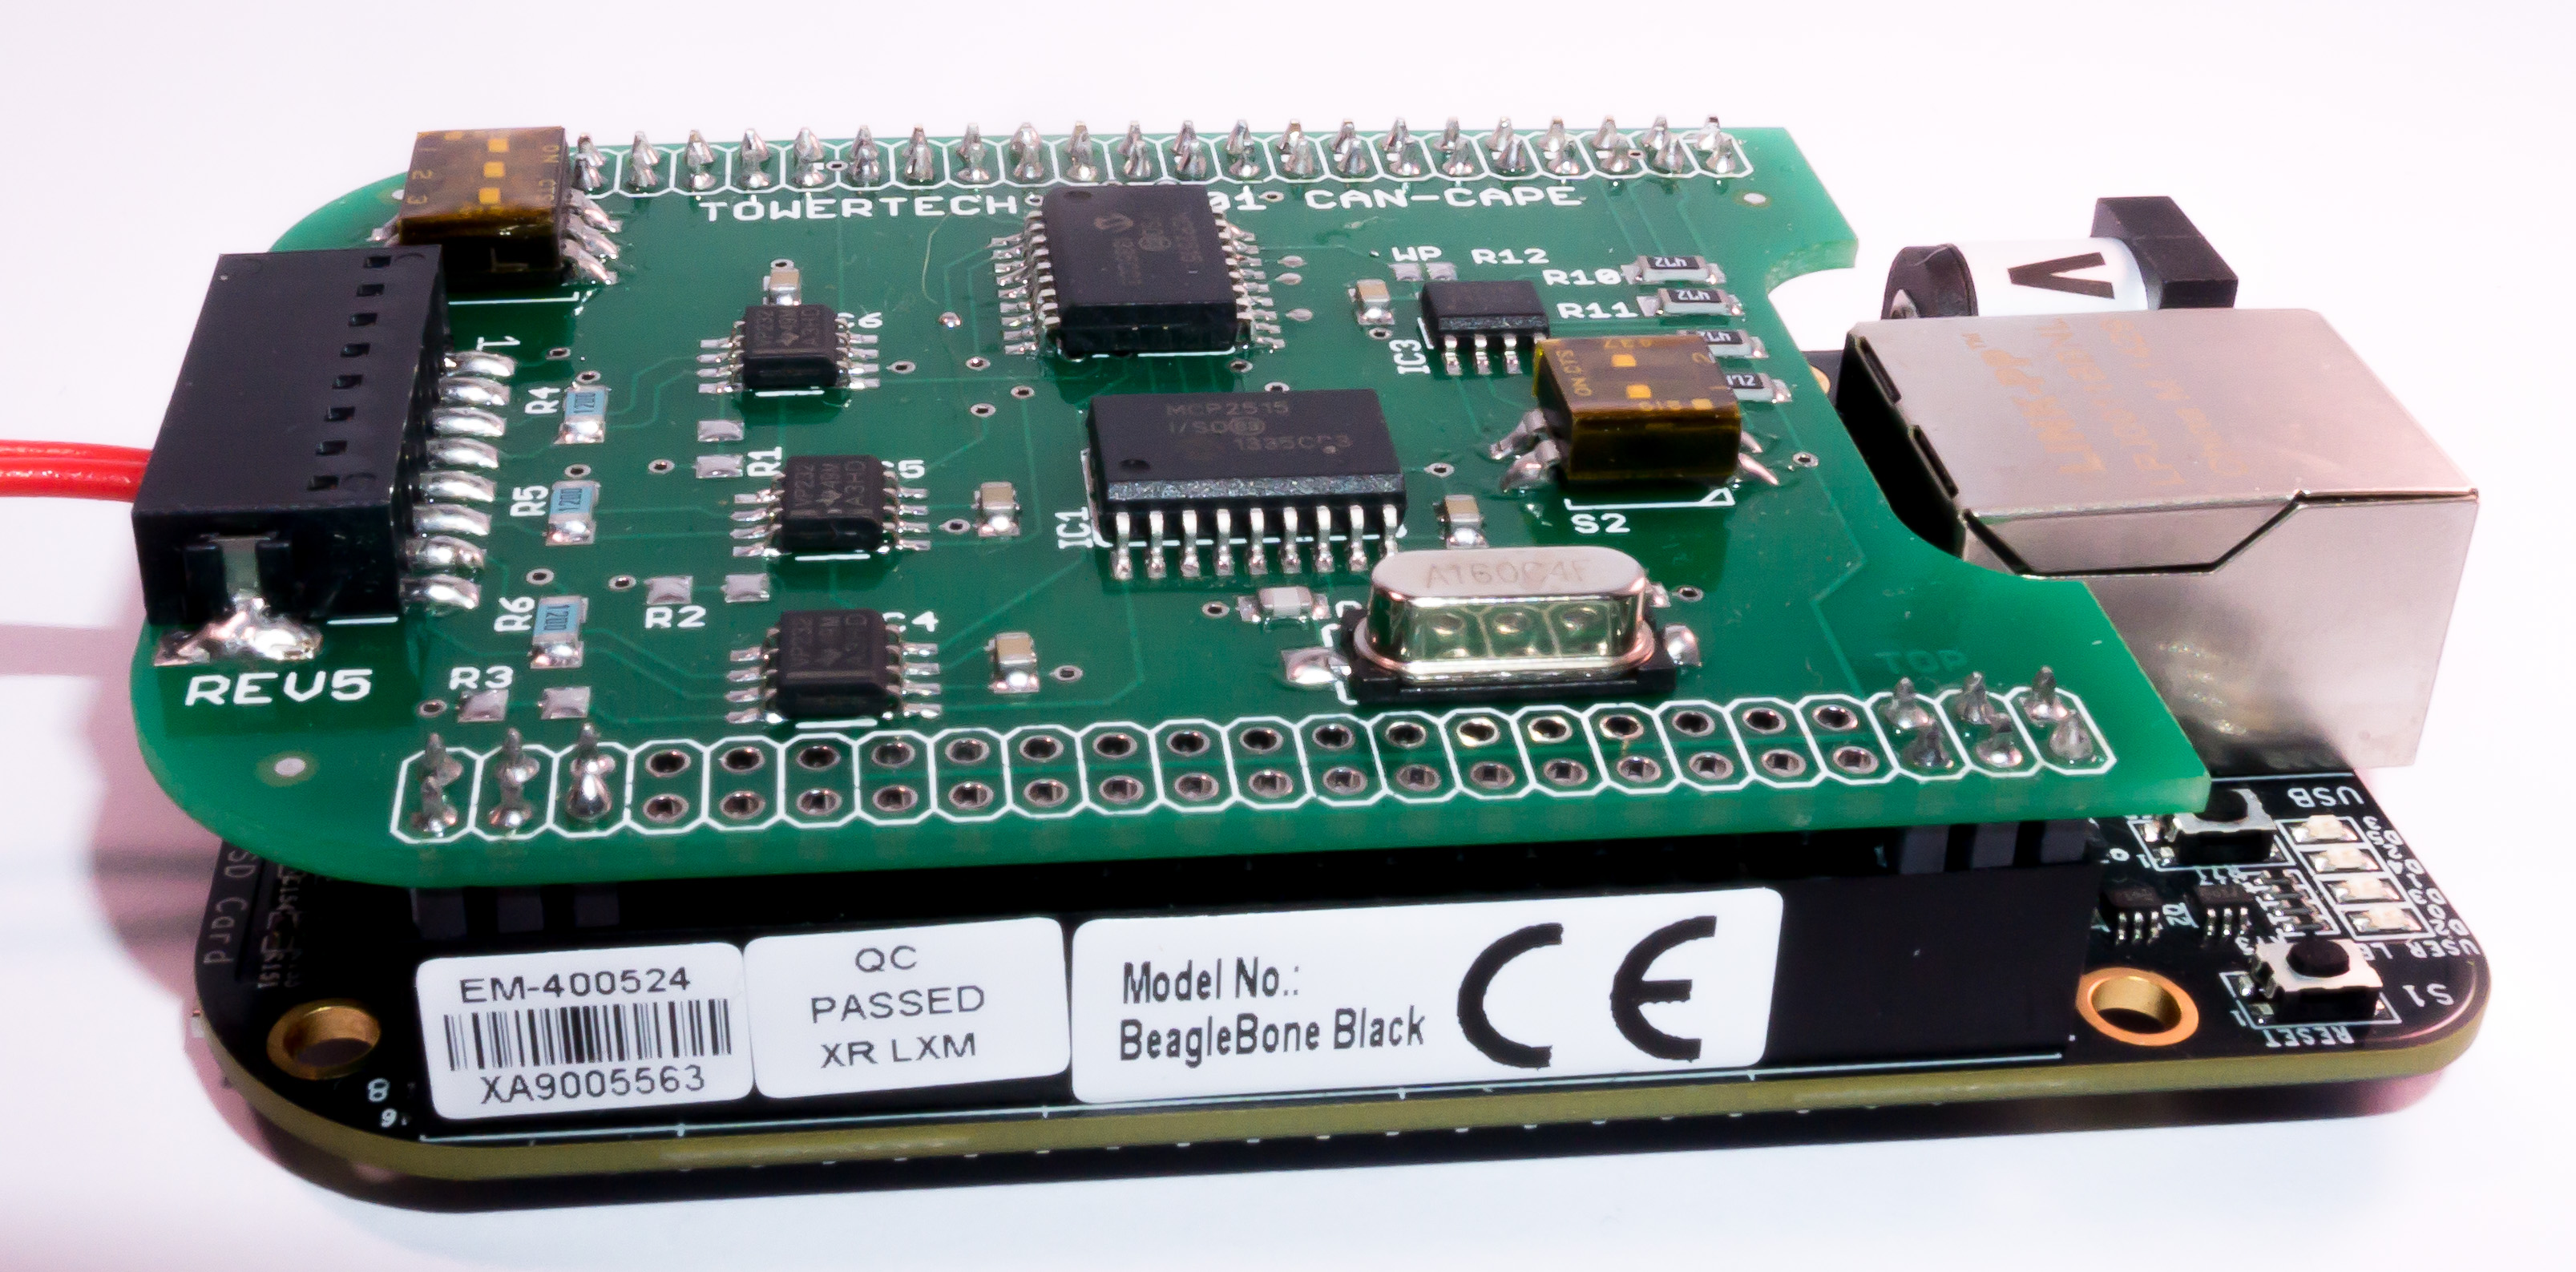
\includegraphics[width=\textwidth]{bilder/foto-3.jpg}
    \caption{Installation CAN-Cape}
    \label{fig:installation_can_cape}
\end{figure}


\section{Install latest Kernel image }
See \url{http://elinux.org/BeagleBoardDebian#Install_Latest_Kernel_Image}

\section{Add default route temporary until next restart}

\begin{lstlisting}
ip route add default via 192.168.7.1
\end{lstlisting}

\section{Add default route permanent}

\subsection{Repair file}

New content for \url{/etc/init.d/led_aging.sh}

\begin{lstlisting}
#!/bin/sh -e
### BEGIN INIT INFO
# Provides:          led_aging.sh
# Required-Start:    $local_fs
# Required-Stop:     $local_fs
# Default-Start:     2 3 4 5
# Default-Stop:      0 1 6
# Short-Description: Start LED aging
# Description:       Starts LED aging (whatever that is)
### END INIT INFO

x=$(/bin/ps -ef | /bin/grep "[l]ed_acc")
if [ ! -n "$x" -a -x /usr/bin/led_acc ]; then
    /usr/bin/led_acc &
fi
\end{lstlisting}


\subsection{Make the default gateway script executable}
\begin{lstlisting}
chmod +x /etc/network/if-up.d/defaultgw
\end{lstlisting}

\subsection{Install post networking script}
\begin{lstlisting}
touch /etc/init.d/initnet && nano /etc/init.d/initnet
\end{lstlisting}

Insert following content:
\begin{lstlisting}
#! /bin/sh
### BEGIN INIT INFO
# Provides: initnet
# Required-Start: $all
# Required-Stop: $all
# Default-Start: 2 3 4 5
# Default-Stop: 0 1 6
# Short-Description: Short script description
# Description: Longer script description.
### END INIT INFO
case "$1" in
        start)
                /sbin/ip route add default via 192.168.7.1
                #/sbin/route add default gw 192.168.7.1 dev usb
                /usr/sbin/ntpdate pool.ntp.org
        ;;
        stop)
                #no-op
        ;;
        *)
                #no-op
        ;;
esac

exit 0

\end{lstlisting}

\begin{lstlisting}
# Make it executable
chmod +x /etc/init.d/initnet
# Test the new Service
insserv -n /etc/init.d/initnet
# Activate new service
insserv /etc/init.d/initnet
\end{lstlisting}

\section{Configure NAT on Ubuntu Host PC}
Add a File namend beaglebonenat (withoud file extension) in \url{/etc/network/if-up.d} and change settings to meet your environment

\begin{lstlisting}
#!/bin/sh -e
#
case "$IFACE" in
    eth3)
        /bin/echo > /proc/sys/net/ipv4/ip_forward 1
        /sbin/iptables -t nat -A POSTROUTING -s 192.168.7.0/24 -o wlan0 -j MASQUERADE
    ;;
esac
\end{lstlisting}

Make the file executable:
\begin{lstlisting}
chmod +x /etc/network/if-up.d/beaglebonenat
\end{lstlisting}


\section{Install TowerTech TT3201 rev 5 on BeagleBone Debian}

\subsection{Get kernel headers}
be sure you have the kernel headers. If your kernel is 3.8.13-bone70,
install as follow:

\begin{lstlisting}
 apt-get update
 apt-get install linux-headers-3.8.13-bone70
\end{lstlisting}

When paket on apt-get install is not found, install Linux Headers for v3.8.13-bone71

\begin{lstlisting}
wget https://rcn-ee.net/deb/wheezy-armhf/v3.8.13-bone71/linux-headers-3.8.13-bone71_1wheezy_armhf.deb 

dpkg -i linux-headers-3.8.13-bone71_1wheezy_armhf.deb 
\end{lstlisting}

\subsection{Invoke the build script}
\begin{lstlisting}
 sh build.sh
 \end{lstlisting}

The installed modules will be in \url{/lib/modules/`uname -r`/extra} and the firmware in \url{/lib.firmware/TT3201*}

\subsection{Configure Beaglebone Cape Manager}
Edit \url{/etc/default/capemgr} to add the TT3201, it should look like this:

\begin{lstlisting}
# Default settings for capemgr. This file is sourced by /bin/sh from
# /etc/init.d/capemgr.sh

# Options to pass to capemgr
CAPE="TT3201-001:05"
\end{lstlisting}


\subsection{Disable HDMI Cape on BeagleBone Black}
Disable the HDMI port by editing uEnv.txt on your \url{/boot} partition.
It should have an entry like this

\begin{lstlisting}
##Disable HDMI
cape_disable=capemgr.disable_partno=BB-BONELT-HDMI,BB-BONELT-HDMIN
\end{lstlisting}


\subsection{Reboot and check cape detection}
Reboot and your cape should be detected automatically, check with
\begin{lstlisting}
cat /proc/cmdline | grep -q "L Bone-Black-HDMI" && echo "ERROR: hdmi NOT disabled"

cat /sys/devices/bone_capemgr.*/slots | grep TT3201
 8: ff:P-O-L Override Board Name,05,Override Manuf,TT3201-001

ip link | grep can[0-9]
 3: can0:  mtu 16 qdisc pfifo_fast state UNKNOWN mode DEFAULT qlen 10
 4: can1:  mtu 16 qdisc noop state DOWN mode DEFAULT qlen 10
 5: can2:  mtu 16 qdisc noop state DOWN mode DEFAULT qlen 10
\end{lstlisting}

\subsection{Check CAN detection}
\begin{lstlisting}
# cat /sys/devices/bone_capemgr.*/slots | grep TT3201
 0: 54:P---L TT3201 CAN Cape,01,TowerTech,TT3201-001

# ip link | grep can[0-9]
3: can0: mtu 16 qdisc pfifo_fast state UNKNOWN mode DEFAULT qlen 10
4: can1: mtu 16 qdisc noop state DOWN mode DEFAULT qlen 10
5: can2: mtu 16 qdisc noop state DOWN mode DEFAULT qlen 10

# dmesg | grep mcp251x
[    7.170413] mcp251x spi1.0: mode 0, irq 259, awake 1, clkout 1, oscillator freq 16000000
[    7.186391] mcp251x spi1.0 can1: probed
[    7.257289] mcp251x spi1.1: mode 0, irq 261, awake 1, clkout 0, oscillator freq 16000000
[    7.371486] mcp251x spi1.1 can2: probed

#  dmesg | grep c_can  
[    6.712145] c_can_platform 481d0000.d_can: invalid resource
[    6.718084] c_can_platform 481d0000.d_can: control memory is not used for raminit
[    6.799197] c_can_platform 481d0000.d_can: c_can_platform device registered (regs=fa1d0000, irq=71)
\end{lstlisting}


\subsection{Install CAN tools}
\begin{lstlisting}
git clone https://github.com/linux-can/can-utils.git
cd can-utils
make
make install
\end{lstlisting}

\subsection{CAN tools examples}
\begin{lstlisting}
ip link set can0 type can bitrate 125000
ip link set can1 type can bitrate 125000

ip link set can0 up
ip link set can1 up


cansend can1 00000104#02aa
candump can0
\end{lstlisting}
